\section{Diagrammes de classes}
	Pour des raisons de lisibilité et de simplification, le diagramme de classe global (fichier diagramme\_classe\_complet.png) se trouve dans un fichier joint dans le $.zip$. Les différentes \og parties \fg du diagramme de classe seront abordées et expliquées une à une.

	\subsection{Organisation générale}
		Les classes principales du jeu sont décrites dans la Figure \ref{fig:classe_general}
		Le jeu comporte une classe mère, qui servira de point d'entrée au programme. Elle appellera les différentes fonctions nécessaire à la création d'une partie (détaillé dans la section \ref{sec:constructeurs}).

		L'attribut \verb|currentGame| du \verb|GameManager| permettra de retrouver toutes les informations utiles à la partie. En effet, elle possèdera en attribut la carte (section \ref{sec:carte}) et la liste des joueurs (qui possèderont la liste de leurs unités).

		\begin{figure}[h!]
			\begin{center}
				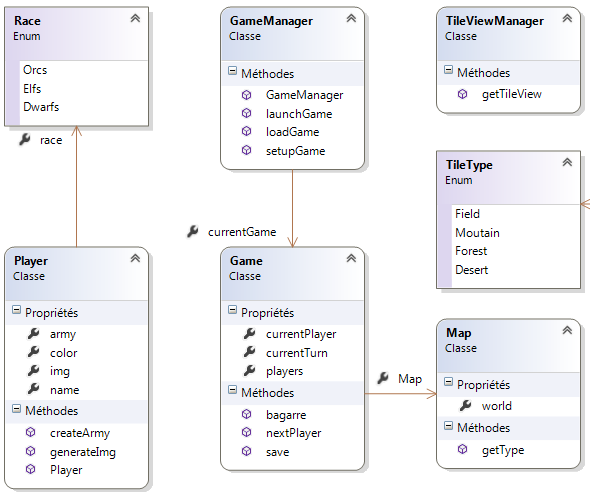
\includegraphics[width=1\textwidth]{figure/classe_general.png}
			\end{center}
			\caption{Ces quelques classes permettent d'avoir une connaissance complète du jeu.}
			\label{fig:classe_general}
		\end{figure}

	\subsection{La carte}
		\label{sec:carte}
		La classe carte (Figure \ref{fig:classe_map}), qui sera générée en début de partie, contiendra un tableau (\verb|world|) de tuiles (\verb|tile|).

		Ces tuiles contiendront plusieurs informations:
		\begin{itemize}
			\item leurs coordonnées ;
			\item la liste des unités étant sur la case.
		\end{itemize}

		Bien que ces informations peuvent déjà être récupérée d'une autre manière, cette répétition de l'information permettra d'accélérer\footnote{Améliorer la complexité des algorithmes.} certaines recherches d'information, au prix d'un surcoût mémoire considéré comme acceptable.

		\`A noter que les tuiles possèdent une information facultative au sujet: il s'agit de l'id de texture. Cela permettra de varier les textures des cases, afin par exemple d'avoir des plaines avec des champs de blés, et des plaines avec des petites maisons dans la prairie.

		\begin{figure}[h!]
			\begin{center}
				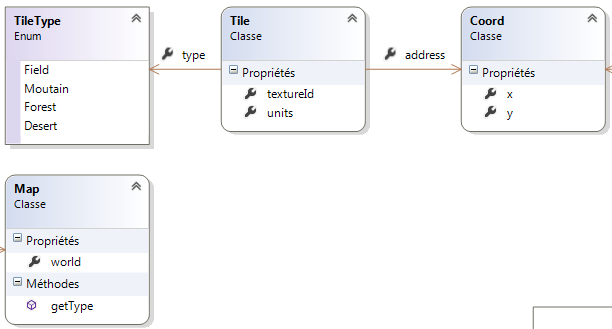
\includegraphics[width=1\textwidth]{figure/classe_map.png}
			\end{center}
			\caption{Les puristes du C auraient pu remplacer la classe Map par un simple tableau bidimensionnel.}
			\label{fig:classe_map}
		\end{figure}

	\subsection{Les unités}
		\label{sec:units}
		Les unités (Figure \ref{fig:unit}) (qui seront générées par la {\textbf factory} UnitFactory) hériteront toutes de la classe abstraite \verb|Unit|.
		Chaque unité aura comme information:
		\begin{itemize}
			\item sa vie actuelle ;
			\item son état actuel ;
			\item sa position ;
			\item ses points de mouvement restants.
		\end{itemize}

		La fonction \verb|move| sera implémentée par chaque descendant de \verb|Unit|. Cela permettra de prendre en compte facilement les spécificités de chaque race lors de leurs déplacement\footnote{Rappelons que le coût de déplacement varie en fonction du type de terrain et de la race}.

		\begin{figure}[h!]
			\begin{center}
				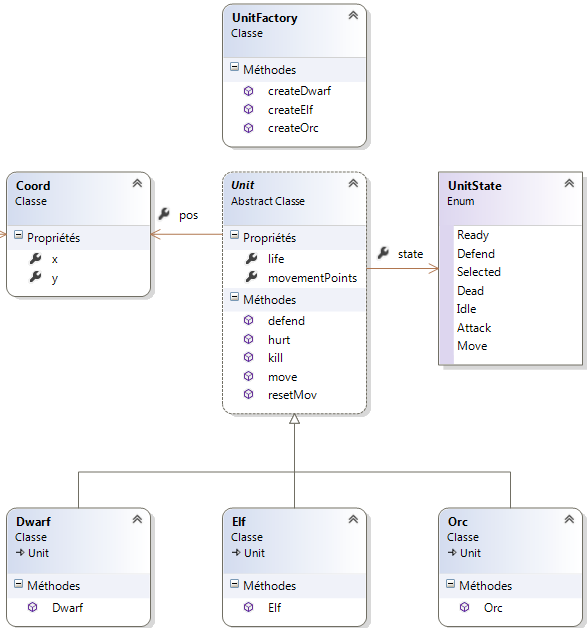
\includegraphics[width=1\textwidth]{figure/classe_unit.png}
			\end{center}
			\caption{La troisième guerre des champignons a mis fin au règne des hommes sur Terre, et par la même occasion, a simplifié le diagramme de classes.}
			\label{fig:unit}
		\end{figure}


	\subsection{Les constructeurs de partie}
		\label{sec:constructeurs}
		Deux cas de figure se présentent au lancement d'une partie. En effet, il peut s'agir d'une toute nouvelle partie, ou bien il suffira de charger une partie enregistrée afin de la continuer.

		Pour faire face à ces différences, une architecture brillante (Figure \ref{fig:classe_builder}), mêlant les patrons \verb|strategy| et \verb|builder|, a été conçue.
		\verb|GameBuilder| sera une classe abstraire, que les différentes stratégies de constructeurs pourront implémenter.
		La fonction \verb|CreateGame| sera surchargée, afin de faciliter l'appel en fonction du besoin. Dans le cas d'une nouvelle partie, il faudra spécifier la taille de la carte et le nom des joueurs. Dans le cas d'un chargement de partie, il faudra spécifier l'id de la partie à charger.

		Lors de la création d'une nouvelle partie, il faudra général une nouvelle carte. Bien qu'externalisée dans une dll c++ externe, il faudra différentes stratégies de génération en fonction de la taille de la carte.


		\begin{figure}[h!]
			\begin{center}
				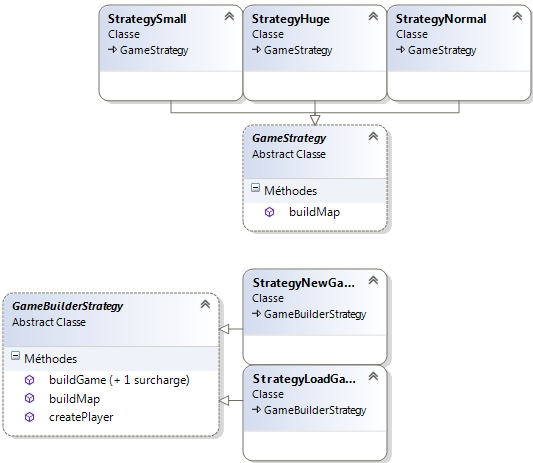
\includegraphics[width=1\textwidth]{figure/classe_builder.png}
			\end{center}
			\caption{Grâce à leur formation bac +8, les constructeurs sont aussi de fins stratèges.}
			\label{fig:classe_builder}
		\end{figure}


	\subsection{La vue}
		Afin de minimiser le coût mémoire, chaque texture de tuile sera chargée une seule fois, puis affichée aux coordonnées nécessaire.
		Le patron de conception \verb|poids mouche| est le plus adapté pour réaliser cette tâche difficile.
		L'utilisation de ce patron est décrite Figure \ref{fig:classe_view}.

		\begin{figure}[h!]
			\begin{center}
				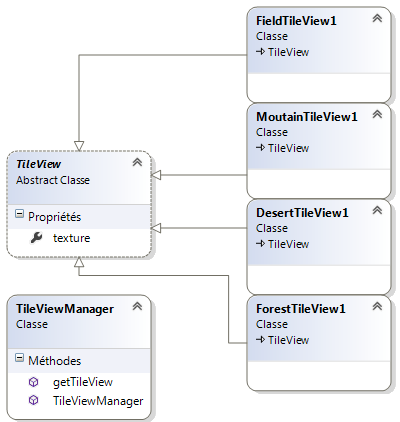
\includegraphics[width=1\textwidth]{figure/classe_view.png}
			\end{center}
			\caption{Afin de simplifier le diagramme, une seule View par type de case est montrée.}
			\label{fig:classe_view}
		\end{figure}
